\documentclass[border=4pt]{standalone}
\usepackage[utf8]{inputenc}
\usepackage[T1]{fontenc}
\usepackage{lmodern}
\usepackage{amsmath,amssymb,mathtools}
\usepackage{tikz}
\usetikzlibrary{calc,decorations.pathreplacing,angles,quotes}
\usepackage{pgfplots}
\pgfplotsset{compat=1.18}
% Figura extraída de la Tarea 11 de Cálculo I (primer semestre).
\begin{document}
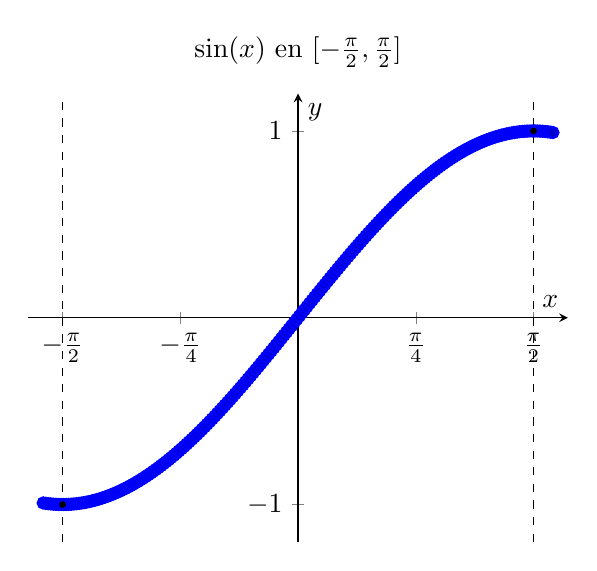
\begin{tikzpicture}
        \begin{axis}[
        domain=-1.7:1.7, samples=200,
        xmin=-1.8, xmax=1.8, ymin=-1.2, ymax=1.2,
        axis lines=middle, xlabel={$x$}, ylabel={$y$},
        xtick={-1.5708,-0.7854,0,0.7854,1.5708},
        xticklabels={\(-\tfrac{\pi}{2}\),\(-\tfrac{\pi}{4}\),0,\(\tfrac{\pi}{4}\),\(\tfrac{\pi}{2}\)},
        ytick={-1,0,1}, title={\(\sin(x)\) en \([-\tfrac{\pi}{2},\tfrac{\pi}{2}]\)}
        ]
        \addplot+[thick]{sin(deg(x))};
        \addplot[only marks,mark=*,mark size=1pt] coordinates {(-1.5708,-1) (1.5708,1)};
        \draw[dashed](axis cs:-1.5708,-1.2)--(axis cs:-1.5708,1.2);
        \draw[dashed](axis cs:1.5708,-1.2)--(axis cs:1.5708,1.2);
        \end{axis}
    \end{tikzpicture}
\end{document}
